\documentclass[11pt,handout]{beamer}

\usepackage{tcolorbox}

% bibliography
\usepackage[backend=biber]{biblatex}
\bibliography{FDS_Seminar_2.bib}

\usepackage[cache=false]{minted}
\usepackage{sourcecodepro}

% isabelle
\newminted{isabelle}{
  frame=single,
  framesep=2mm,
  fontsize=\scriptsize,
  mathescape
}

\newminted{prolog}{
  frame=single,
  framesep=2mm,
  fontsize=\scriptsize,
  mathescape
}

\makeatletter
\AtBeginEnvironment{minted}{\dontdofcolorbox}
\def\dontdofcolorbox{\renewcommand\fcolorbox[4][]{##4}}
\makeatother

\usepackage{graphicx}
\usepackage{amsmath}
\usepackage{bussproofs}
\usepackage{mathpartir}
\usepackage{prooftrees}
\usepackage{color}

% remove the Figure :
\usepackage{caption}
\captionsetup{figurename=}

\usepackage{algorithmicx}
\usepackage{algpseudocode}

\graphicspath{{img/}}

\usetheme{CambridgeUS}

\author{Sylvain Julmy}
\title[FDS Seminar]{Seminar Foundations of Dependable Systems}
\date{\today}

\AtBeginSection[]
{
  \begin{frame}
    \frametitle{Table of Contents}
    \tableofcontents[currentsection]
  \end{frame}
}

\begin{document}

\maketitle


\begin{frame}[allowframebreaks]
  \frametitle{Plan for today}
  {
    \small
    \tableofcontents
  }
\end{frame}

\begin{frame}
  \frametitle{Interactive Theorem Prover}
  Interactive Theorem Prover (ITP) becomes a more common way of establishing the
  correctness of software and mathematical proofs :
  \begin{itemize}
  \item Compilers
  \item Operating Systems
  \item Kepler Conjecture
  \item Feit-Thompson Theorem
  \end{itemize}
  \note[item]{Kepler Conjecture : stack of sphres in the plan has a density of 74\%.}
  \note[item]{Feit-Thompson Theorem : every finite group of odd order is solvable.}
\end{frame}

\begin{frame}
  \frametitle{Interactive Theorem Prover}
  ITPs enable users to interact with a proof system and guide a proof. They also
  support automation in terms of user-provided tactics.
\end{frame}

\section[Typed MIL]{Typed meta-interpretive learning}

\subsection[Introduction]{Introduction and context}

\begin{frame}[fragile]
  \frametitle{Introduction and context}
  Ability to learn and re-apply proof strategies would significantly increase
  the  productivity and effectiveness.

  \vspace*{1cm}

  \begin{isabellecode}
    lemma K: A -> B -> A
    proof
      assume A
      show B -> A
      proof
        show A by fact
      qed
    qed
  \end{isabellecode}

  \note{This is a small example of a proof for the K combinator with Isabelle.
    There are multiple proof and sub-proof which could be reuse.}
\end{frame}

\begin{frame}
  \frametitle{Introduction and context : problem}
  The user must often manually provide guidance and proofs, often group into
  famillies, such that, once the user has discharged one proof, discharging the
  other is simpler.

  \vspace*{1cm}

  The idea is to learn and reapply proof strategies from a few examples.
\end{frame}

\begin{frame}
  \frametitle{Introduction and context}
  Previous work to learn proof strategies has only attempted to extract general
  strategies from a large corpus of proofs.
  \note{
    Previous work to learn proof strategies has only attempted to extract general
    strategies from a large corpus of proofs.
  }

  \vspace*{1cm}
  
  They are not addressing the desirable extraction of local strategies. Which
  was the motivation for developing the \texttt{PSGraph} language.
\end{frame}

\begin{frame}[fragile]
  \frametitle{Overview of the approach}
  \begin{figure}[h]
    \centering
    \frame{
      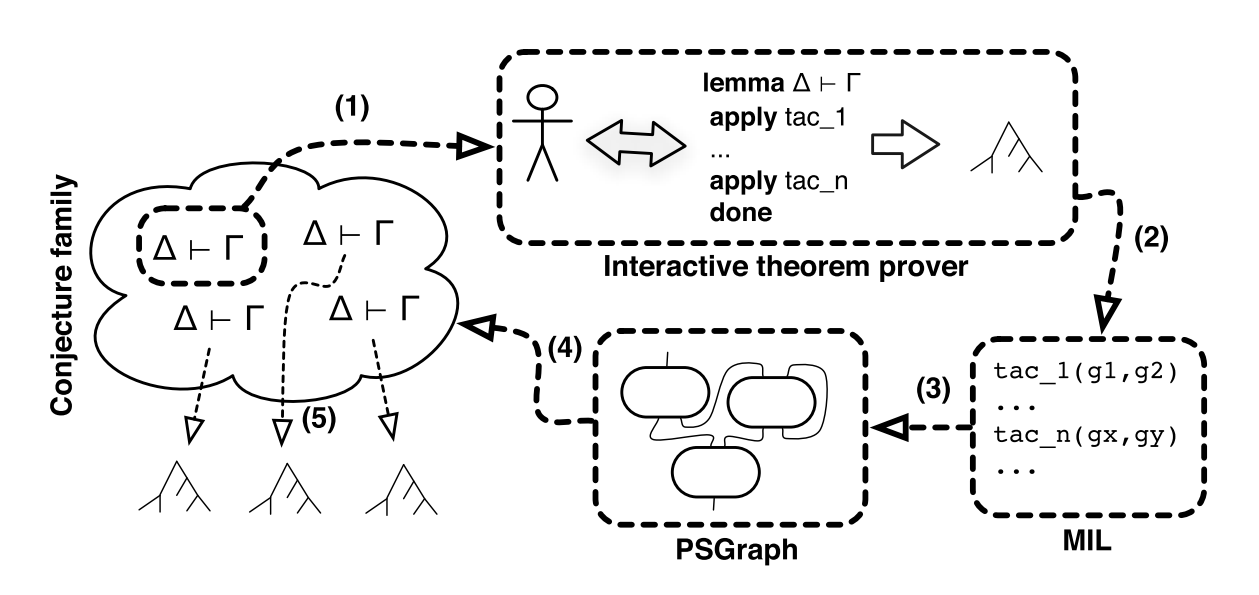
\includegraphics[width=0.9\textwidth]{overview_tmil}
    }
    \caption{Overview of the approach.}
  \end{figure}
  \note[item]{A user selects one (or a few) conjectures from a “conjecture family”
    and guides the proof as normal (using a proof script) in an ITP system. This will
    generate a proof tree.}
  \note[item]{Metagol is used to learn a proof strategy from the proof tree.}
  \note[item]{The proof tree is translated to PSGraph.}
  \note[item]{We apply the proof strategy to the other conjectures of the familly.}
  \note[item]{Which will generate new proof trees.}
\end{frame}

\begin{frame}
  \frametitle{Goal}
  \begin{enumerate}
  \item Show that MIL can learn proof strategies for the PSGraph language.
  \item Extend MIL with types.
  \item Demonstrate that ``typed MIL learns more deterministic proof strategies than untyped MIL''.
  \item Show that introducing dependent learning reduces the time taken to learn a strategy.
  \end{enumerate}
\end{frame}

\subsection[PSGraph]{PSGraph}

\begin{frame}
  \frametitle{PSGraph}
  The language aims to represent proof strategies as graphs, where proof tactics
  are represented by boxes and goal information by predicate which label the
  wires.
\end{frame}

\begin{frame}[fragile]
  \frametitle{ITP and PSGraph}
  \begin{figure}[h]
    \centering
    \frame{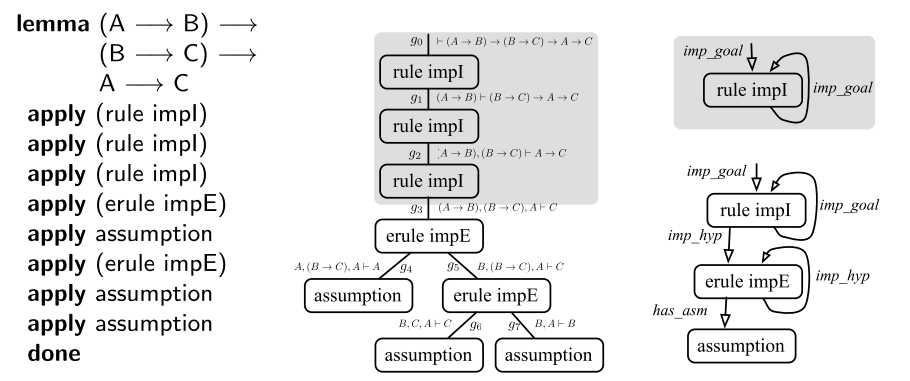
\includegraphics[width=0.9\textwidth]{left_to_right_example}}
    \caption{Left to right: Isabelle proof script; proof tree; and strategy as PSGraph.}
  \end{figure}
  \note[item]{
    To develop theories and proofs, a user works with a proof script. The proof
    shown illustrates a proof of a conjecture in propositional logic.
    The first line states the conjecture to be proved, and is followed
    by a sequence of apply commands before the proof is closed by done.
  }
  \note[item]{
    For this specific proof, the idea is to remove all the implication in the
    conclusion by the deductiom lemma. Then remove all implication in the
    hypothesis by applying the assumption. At the end, everything can be proven
    by the assumption tactics.
  }
  \note[item]{
    The apply (tactics) take a lemma and a proof methods.
  }
\end{frame}

\begin{frame}
  \frametitle{ITP and PSGraph}
  By proving a single conjecture a user will develop a proof strategy that he
  can reapply across a family of similar conjectures.

  \note[item]{Such families are common, either as separate conjectures or as
    sub-goals within a single conjecture.}

  \vspace*{1cm}

  The strategies are normally in the head of a user, although an expert may
  manually encode them as tactics, the goal is to help automate the extraction
  and application of such strategies.
\end{frame}

\begin{frame}
  \frametitle{ITP and PSGraph}
  A proof strategy needs to include procedural information about which tactics
  to apply, the type of goal and progress made to show how a goal should evolve.
  \note[item]{That's why PSGraph has been developed. The other system are
    lacking the last two points.}
  
  \vspace*{1cm}

  A directed labelled graph is used to capture proof strategies : the boxes of
  the graph contain the tactics, wires are labelled by wire predicates.

  \note[item]{Wire predicates : predicates to describe why a sub-goal should be
    on a given wire.}

  \vspace*{1cm}
  
  A graph is evaluated as a flow graph, where a goal
  flows between tactics on a directed edge if the predicate on the edge holds for
  that particular goal.
\end{frame}

\begin{frame}[fragile]
  \frametitle{ITP and PSGraph}
  \begin{figure}[h]
    \centering
    \frame{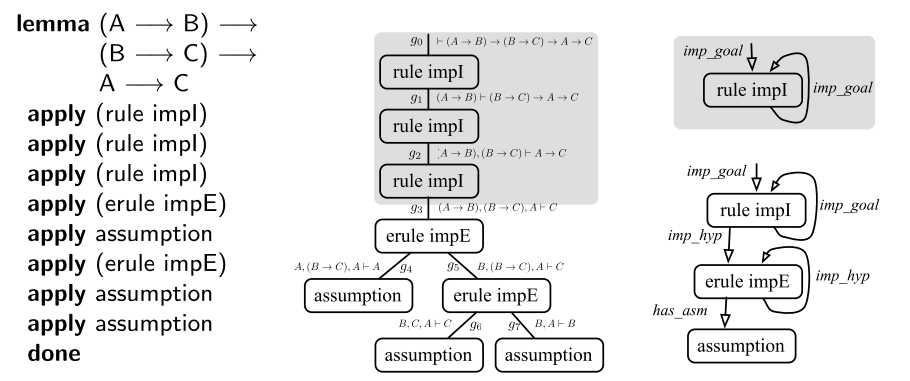
\includegraphics[width=0.9\textwidth]{left_to_right_example}}
    \caption{Left to right: Isabelle proof script; proof tree; and strategy as PSGraph.}
  \end{figure}
  \note{
    Here, imp goal is a predicate that holds if the conclusion is an
    implication; imp hyp is a predicate that holds if the hypothesis is an implication
    and the conclusion is not; while has assm holds if the conclusion is present in the
    hypotheses. The remainder of the paper addresses learning of PSGraphs from a
    small set of examples. The shaded parts of Fig. 2 highlight a sub-proof (middle),
    which we can learn a sub-strategy from (right). We will return to this below.
  }
\end{frame}

\subsection[MIL]{Meta-Interpretive Learning : MIL}

\begin{frame}[fragile]
  \frametitle{Metagol}
  The framework is built on top of MIL by using Metagol.
  
  Metagol\cite{metagol} is an inductive logic programming (ILP) system based on
  meta-interpretive learning.

  \note[item]{
    Whereas a standard Prolog meta-interpreter
    attempts to prove a goal by repeatedly fetching first-order clauses whose heads
    unify with a given goal, a MIL learner attempts to prove a set of goals by
    repeatedly fetching higher-order metarules (e.g. P(X, Y) ← Q(Y,X)) whose
    heads unify with a given goal.
  }
  \note[item]{
    The basic idea is to process the unification on the predicate and not on the argumments.
  }
\end{frame}

\begin{frame}[fragile]
  \frametitle{}
  \begin{prologcode}
    %% first-order background knowledge
    mother(ann,amy).
    mother(ann,andy).
    mother(amy,amelia).
    mother(linda,gavin).
    father(steve,amy).
    father(steve,andy).
    father(gavin,amelia).
    father(andy,spongebob).

    %% predicates that can be used in the learning
    prim(mother/2).
    prim(father/2).
  \end{prologcode}
\end{frame}

\begin{frame}[fragile]
  \frametitle{}
  \begin{prologcode}
    %% metarules
    metarule([P,Q],([P,A,B]:-[[Q,A,B]])).
    metarule([P,Q,R],([P,A,B]:-[[Q,A,B],[R,A,B]])).
    metarule([P,Q,R],([P,A,B]:-[[Q,A,C],[R,C,B]])).

    %% learning task
    a :-
    %% positive examples
      Pos = [
        grandparent(ann,amelia),
        grandparent(steve,amelia),
        grandparent(ann,spongebob),
        grandparent(steve,spongebob),
        grandparent(linda,amelia)
        ],
    %% negative examples
      Neg = [
        grandparent(amy,amelia)
      ],
      learn(Pos,Neg).
  \end{prologcode}
\end{frame}

\begin{frame}[fragile]
  \frametitle{Metagol : output}
  \begin{prologcode}
    % clauses: 1
    % clauses: 2
    % clauses: 3
    grandparent(A,B):-grandparent_1(A,C),grandparent_1(C,B).
    grandparent_1(A,B):-mother(A,B).
    grandparent_1(A,B):-father(A,B).
  \end{prologcode}

  \note[item]{The predicate grandparent/2 is invented and corresponds to
    the parent relation.}
\end{frame}

\begin{frame}[fragile]
  \frametitle{Metarules}
  Metagol requires higher-order metarules to define the form of clauses
  permitted in a hypothesis.
  \begin{prologcode}
    metarule([P,Q,R],([P,A,B]:-[[Q,A,C],[R,C,B]])).
  \end{prologcode}
  \note[item]{The list of symbols in the first argument denote the existentially
    quantified variables which Metagol will attempt to find substitutions for
    during the learning.}
  Users need to supply Metarules. Work is in progress\footnote{at the time of
    this paper} for automatically identifying the necessary metarules.
\end{frame}

\subsection[Adding types]{Adding types}

\begin{frame}
  \frametitle{Typed Meta-Interpretive Learning}

  \begin{tcolorbox}[colback=blue!5!white,colframe=blue!85!black,title=Typed Meta-Interpretive Learning]
    Typed MIL extends MIL by labelling each predicate $P$ with a constant $t$
    representing its type. This is written $P : t,$ such that $P(X,Y)$
    becomes $P : t(X, Y)$. The type is treated as an extra constant argument,
    thus $P : t(X,Y)$ is internally represented as $P(t,X, Y)$.
  \end{tcolorbox}
\end{frame}

\begin{frame}
  \frametitle{Learning cases}
  Learning PSGraphs from example proofs can be reduced to two mutually de-
  pendent learning problems :
  \begin{enumerate}
  \item learning a graph’s structure.
  \item learning suitable wire predicates.
  \end{enumerate}

  Previous learning attempts have simplified the problem to just the first
  point.
  \note[item]{with the learned strategies lacking explanation resulting in,
    as our experiments show, a higher branching factor and thus slower search.}
\end{frame}

\begin{frame}
  \frametitle{Learning cases}
  
  These two problems have different features :
  
  \begin{enumerate}
  \item requires learning clauses which can be translated into a graph with wire predicates
  \item needs a large search space in order to learn unknown predicates.
  \end{enumerate}

  Working with HOL this includes arbitrary recursive functions. In typed MIL we
  can control the structure of what is learned with metarules, and use types to
  separate the learning problems.
\end{frame}

\begin{frame}
  \frametitle{Used metarules}
  Typed MIL use the following metarules :
  \begin{itemize}
  \item $Lift$ : construct a PSGraph consisting of a single node (tactic) and a
    labelled input edge.
  \item $Chain$ : sequentially composes two such PSGraphs to find a larger strategy.
  \item $Loop$ : introduce iteration.
  \item $WChain$ : to learn wire predicate in chain.
  \item $WBin$ : to learn binary wire predicate.
  \end{itemize}
\end{frame}

\begin{frame}[fragile]
  \frametitle{Lift}
  
  \begin{align*}
    PSGraph(psgraph,g_x,g_y) \leftarrow & predicate(wpred,g_x),\\
                                        & tactic(tactic,g_x,g_y).
  \end{align*}

    \note[item]{Lift : Metagol finds the appropriate tactic clause in
    the background information, labelled with type tactic, and tries to find a clause
    of type wpred to define the wire predicate on the input edge. If a suitable $wpred$
    clause can be found in the background information it will be inserted, otherwise
    Metagol will use further metarules (such as WChain and WBin in Fig. 4) to
    attempt to find a suitable definition from the available information. Thus we
    find that the node in the proof tree has been ”lifted“ into the PSGraph.}
\end{frame}

\begin{frame}[fragile]
  \frametitle{Chain}

  \begin{align*}
    PSGraph(psgraph,g_x,g_y) \leftarrow & subgraph_1(psgraph,g_x,g_z),\\
                                        & subgraph_2(psgraph,g_z,g_y).
  \end{align*}
  
  \note[item]{Chain : Chain sequentially composes two such psgraphs to find a larger strategy,
    which are themselves found using the Lift rule. Starting at an edge represnting
    some goal gx on a proof tree and terminating at gy via some intermediate goal
    gz, the resulting PSGraph would be.}
\end{frame}

\begin{frame}[fragile]
  \frametitle{Loop}

  \begin{align*}
    PSGraph\_base(psgraph, gx, gy) \leftarrow & predicate(wpred, gx), tactic(tactic, gx, gy).\\
    PSGraph\_rec(psgraph, gx, gy)  \leftarrow & PSGraph\_base(psgraph, gx, gz),\\
                                              & PSGraph\_rec(psgraph, gz, gy).
  \end{align*}
  
  \note[item]{Loop : Loop introduces iteration, which is represented in PSGraph
    as an additional output edge from a node looping back round to act as an
    additional input to that node. Strategies learned using Loop will always
    have two clauses: a base case in which the tactic is applied once and a
    recursive case where it is applied repeatedly.}
\end{frame}

\begin{frame}[fragile]
  \frametitle{WBin and WChain}
  \begin{align*}
    P : wpred(x) \leftarrow Q : gdata(x, z), R : gdata(x, z).
  \end{align*}
  \begin{align*}
    P : wpred(x) \leftarrow Q : gdata(x, z).
  \end{align*}
\end{frame}

\begin{frame}[fragile]
  \frametitle{Metarules}
  \begin{figure}[h]
    \centering
    \frame{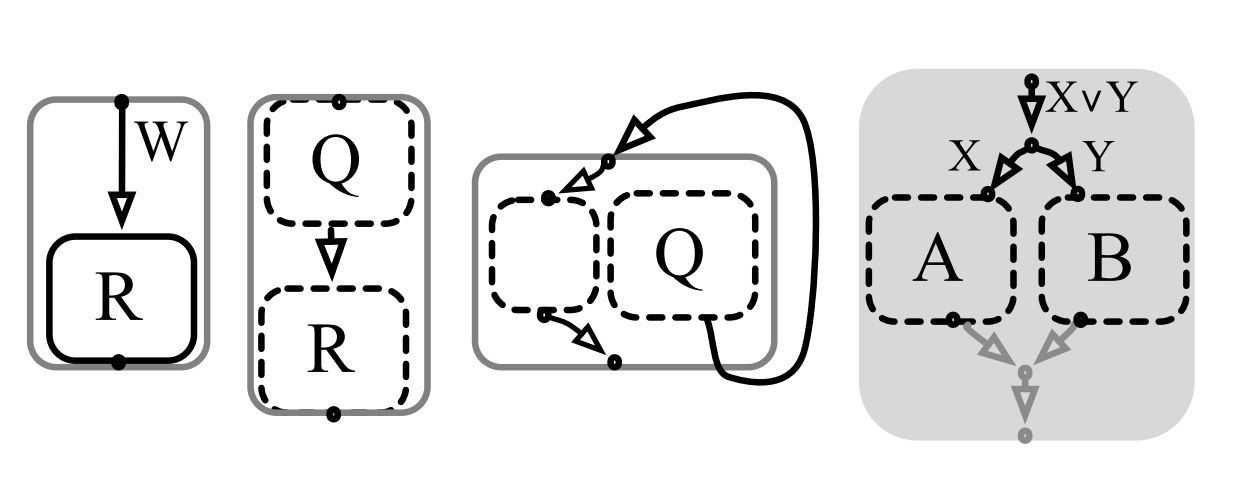
\includegraphics[width=0.8\textwidth]{metarules}}
    \caption{Metarules in PSGraph.}
  \end{figure}
  \note[item]{
    A graphical view is given in Fig. 5, with
    the outer grey lines indicate the learnt PSGraph in each case and stippled boxes
    indicating that the boxes are of type psgraph, meaning they may represent a
    sub-graph. The dots indicate where input and output wires are plugged.
  }
  \note[item]{
    there may be multiple clauses
    describing a learnt PSGraph and without loss of generality we assume there are
    two clauses, A and B, as in Fig. 5 (shaded). By the IH we know that both A
    and B have a single input with predicates X and Y respectively. Here, A and
    B are put side by side and an identity box (which does nothing) is added with
    one input. This has predicate $X \vee Y$. The outputs are then sent to A and B
    using their respective types. They will not have output wires. If this composed
    box is chained to another component R, which has input wire with predicate Z,
    then the output of all non-recursive components are combined to an idenity box
    which is plugged to R. Any wires introduced will have predicate R.
  }
\end{frame}

% \begin{frame}
%   \frametitle{Theorem}
%   \begin{tcolorbox}[colback=blue!5!white,colframe=orange!85!white]
%     A PSGraph constructed using Lift, Chain and Loop will have a
%     single typed input, no outputs and all wires will be labelled with appropriate
%     predicates.
%   \end{tcolorbox}
% \end{frame}

% \begin{frame}
%   \frametitle{Theorem}
%   \begin{tcolorbox}[colback=blue!5!white,colframe=orange!85!white]
%     The translation of Lift, Chain and Loop into a PSGraph of Fig.
%     5 will generate an unique PSGraph.
%   \end{tcolorbox}
% \end{frame}

% \begin{frame}
%   \frametitle{Theorem}
%   \begin{tcolorbox}[colback=blue!5!white,colframe=orange!85!white]
%     If all given tactics terminate, then a learnt PSGraph will either
%     fail or terminate for any input.
%   \end{tcolorbox}
% \end{frame}

% TODO page 24,25,26,27

\subsection[Encoding of a proof tree]{Encoding of a proof tree}

\begin{frame}
  \frametitle{Proof tree}
  The metarules are used to learn proof strategies from an encoding of a proof
  tree.

  \vspace*{1cm}

  A sub-tree is defined in terms of its boundary within a proof tree.
\end{frame}

\begin{frame}[fragile]
  \frametitle{Proof tree encoding}

  \begin{figure}[h]
    \centering
    \frame{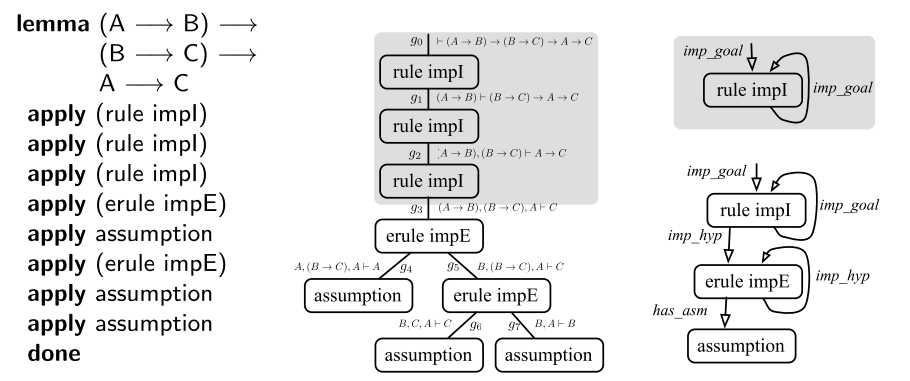
\includegraphics[width=0.8\textwidth]{left_to_right_example}}
    \caption{Previous example.}
  \end{figure}

  \begin{align*}
    rule\_impI : tactic(g0, g1). rule\_impI : tactic(g1, g2). rule\_impI : tactic(g2, g3).
  \end{align*}

  \note[item]{To illustrate, (g0, [g3]) and (g2, [g4, g5]) are valid subtree
    boundaries while (g2, [g4, g7]) is not as g4 and g7 are not equidistant from
    g2 (and there are other nodes which are).}
  \note[item]{
    From the Lift rule, we see that a tactic R will have the form R : tactic(X, Y).
    For example, the tactic rule impI will be encoded as rule impI : tactic. Our
    running proof sub-tree is encoded as : formula
  }
\end{frame}

\begin{frame}[fragile]
  \frametitle{Proof tree encoding}

  \begin{figure}[h]
    \centering
    \frame{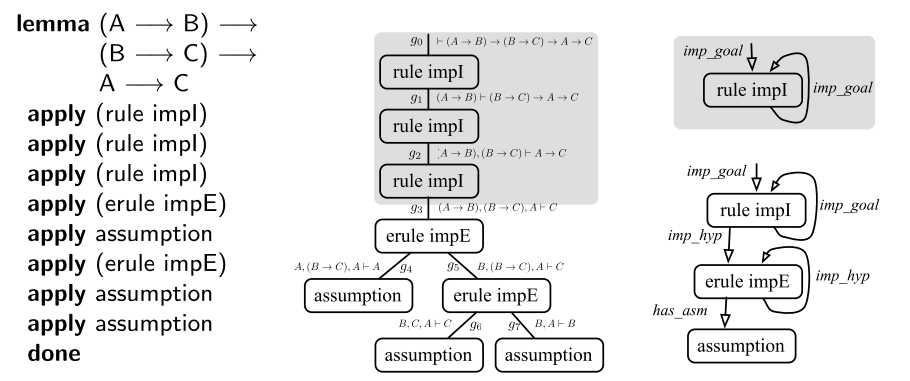
\includegraphics[width=0.8\textwidth]{left_to_right_example}}
    \caption{Previous example.}
  \end{figure}

  \begin{align*}
    erule\_impE : tactic(g3, g4). erule\_impE : tactic(g3, g5).
  \end{align*}

  \note[item]{
    If a tactic produces two sub-goals then two predicates are created, e.g. the
    step that turns g3 into g4 and g5 is represented by the clauses.
  }
  \note[item]{
    For tactics that do not produce any sub-goals (e.g. assumption), a dummy goal
    is created with no goal information in order to preserve the syntax. We call such
    goals terminal.
  }
\end{frame}

\begin{frame}[fragile]
  \frametitle{Proof tree encoding}

  \[
    g_2 \text{ is } A \to B, B \to C \vdash A \to C
  \]

  These terms are projected from the goals by $hyp:gdata$ and $concl:gdata$.

  \begin{align*}
    has\_asm : wpred(G) \leftarrow hyp:gdata(G,T), concl:gdata(G,T).
  \end{align*}
  
  \note[item]{
    All other goals contain a set of hypotheses and a conclusion, which
    we provide projections of.
  }
\end{frame}

\begin{frame}
  \frametitle{Isabelle encoding}
  Isabelle stores terms as typed lambda expressions, using De Bruijn indices.

  \vspace*{1cm}

  \begin{mathpar}
    b(I)\ c(S)\ v(S)\ app(T, U)\ lambda(V, T)\ exists(T)\ forall(Y)
  \end{mathpar}
\end{frame}

\begin{frame}
  \frametitle{Encoding for $g_2$}

  \begin{align*}
    hyp &: gdata(g2, app(app(c(\to), c(a)), c(b))).  \\
    hyp &: gdata(g2, app(app(c(\to), c(b)), c(c))).  \\
    concl &: gdata(g2, app(app(c(\to), c(a)), c(c))).\\
  \end{align*}
\end{frame}

\begin{frame}
  \frametitle{Advantages over machine learning techniques}
  An advantage that ILP techniques have over machine learning techniques is that
  we can enrich the background clauses and use this to guide and simplify
  learning.

  \note[item]{ML techniques used in related work.}

  \vspace*{1cm}

  For example, definitions to extract the top level symbol in a
  conclusion or hypothesis are provided :

  \begin{align*}
    topsymbol : gdata(G,X) & \leftarrow concl : gdata(G, app(app(X, A), B)).\\
    hypsymbol : gdata(G,X) & \leftarrow hyp : gdata(G, app(app(X, A), B)).
  \end{align*}
\end{frame}

\begin{frame}
  \frametitle{Proof tree encoding}
  \begin{tcolorbox}[colback=blue!5!white,colframe=orange!85!white]
    In a proof-tree encoding each step of the proof tree is encoded as a
    relation of type tactic, with associated encoding of the goal information in
    terms of their hypotheses and conclusion.
  \end{tcolorbox}
\end{frame}

\begin{frame}
  \frametitle{Atomic term operator}
  \begin{tcolorbox}[colback=blue!5!white,colframe=orange!85!white]
    The following clauses are atomic term operators :
    \begin{align*}
      &const : gdata(c(X)) &  var : gdata(v(X)) \\
      &bound : gdata(b(X)) & left : gdata(app(X, Y),X) \\
      &right : gdata(app(X, Y), Y) & into : gdata(forall(X),X) \\
      &into : gdata(exists(X),X) & into : gdata(lambda(V,X),X)
    \end{align*}
  \end{tcolorbox}
\end{frame}

\begin{frame}
  \frametitle{Atomic term operator : example}
  The $X$ in $app(app(X, A), B)$ is projected by two consecutive $left : gdata$
  application.
\end{frame}

\begin{frame}
  \frametitle{Learning problem}
  \begin{tcolorbox}[colback=blue!5!white,colframe=orange!85!white]
    In typed MIL of PSGraph a binary relation of type PSGraph is learned where
    the background information at least contains encodings of one or more proof
    trees together with atomic term operators, and the given examples are one or
    more subtree boundaries of the encoded proof trees.
  \end{tcolorbox}

  When using sub-trees and not the full trees we can learn sub-strategies and,
  as discussed later, we can apply dependent learning to learn increasily larger
  sub-strategies.

  \note[item]{
  When using sub-trees and not the full trees we can learn sub-strategies and,
  as discussed later, we can apply dependent learning to learn increasily larger
  sub-strategies.
}
\end{frame}

\begin{frame}[fragile]
  \frametitle{Learning problem : example}
  \begin{figure}[h]
    \centering
    \frame{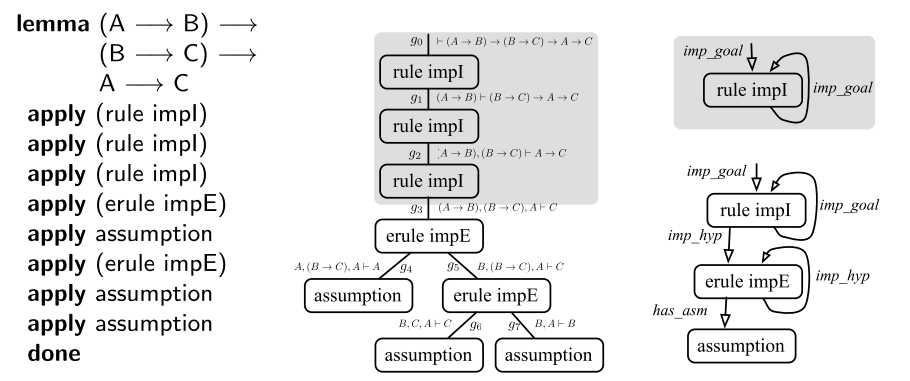
\includegraphics[width=0.8\textwidth]{left_to_right_example}}
    \caption{Previous example.}
  \end{figure}

  \note[item]{
    Returning to the previous example, the shaded part. Metagol will use a metarule
    of the $psgraph$ type as this is the type given for $rule\_imp$.
  }

  \note[item]{
    In our case, Loop will
    trigger learning of the “loop body” $Q : psgraph(x, z)$. Here, Lift is
    applied using the background information $rule impI : tactic(g0, g1)$ to
    generate rule $impI : tactic(A,B)$. Metagol must also find a wire predicate,
    of type wpred for the input.
  }
  
  \note[item]{
    Since no wpred clauses are given in the background information,
    Metagol must invent one. $WBin$ instantiates $B$ in topsymbol :
    $gdata(A,B)$ to $c(imp)$, which is the top symbol of the conclusion of
    $g0$. This invented predicate is called $imp goal : wpred$ and the
    invented graph component is called simpI:psgraph. In order to reach $g_3$,
    and end the loop (base case), Lift is again applied to find a clause with
    body identical to $simpI:psgraph$.
  }
\end{frame}

\begin{frame}
  \frametitle{Learning problem : example}
  \begin{align*}
    rimpI : psgraph(A,B) & \leftarrow simpI : psgraph(A,C), rimpI : psgraph(C, B). \\
    rimpI : psgraph(A,B) & \leftarrow imp goal : wpred(A), rule impI : tactic(A,B).\\
    simpI : psgraph(A,B) & \leftarrow imp goal : wpred(A), rule impI : tactic(A,B).\\
    imp goal : wpred(A)  & \leftarrow topsymbol : gdata(A, c(imp)).
  \end{align*}
  \note[item]{ The learnt program then becomes.}
\end{frame}

\begin{frame}[fragile]
  \frametitle{Learning problem : example}
  \begin{figure}[h]
    \centering
    \frame{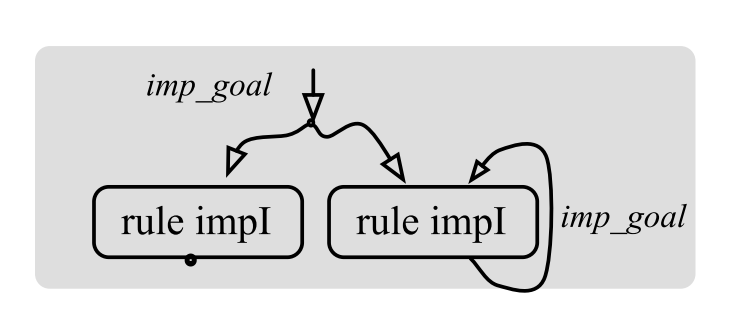
\includegraphics[width=0.8\textwidth]{example}}
    \caption{PSGraph encoding for the example.}
  \end{figure}
  \note[item]{
    A PSGraph encoding of this, following our described translation, is given in Fig
    6. Our metarules have taken a more “functional view” of iteration, meaning
    the solution deviates from the example strategy of Fig 2 as there is a separate
    base and step case, which are identical here.
  }
  \note[item]{
    When considered as a sequence of tactics, we note that proof strategies do
    not always terminate in ITP. If the Loop metarule is naively applied, an infinite
    sequence of tactics may be introduced. We address this by evaluating the sub-
    goals generated by each iteration of the tactic(s) on the recursive node, and define
    termination in terms of an ordering > over the goals. Note that we cannot derive
    a general ordering for all possible conjectures. With the exception of proof by
    contradiction, we can use the total number of symbols for propositional and
    predicate logic addressed in this paper. Let symbcount be the total number of
    symbols (e.g. ∀ or →) for a goal : $G1 >- G2 ← symbcount(G1) > symbcount(G2)$.
  }
\end{frame}

\begin{frame}[fragile]
  \frametitle{Architecture}
    \begin{figure}[h]
    \centering
    \frame{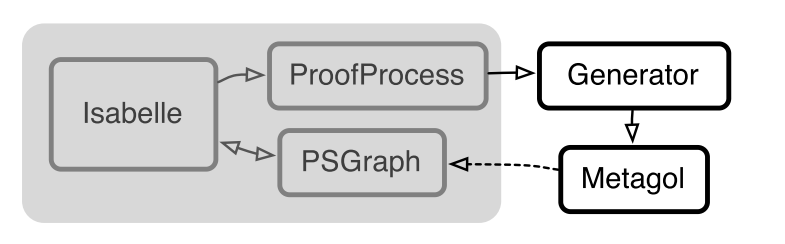
\includegraphics[width=0.8\textwidth]{arch}}
    \caption{Tool architecture.}
  \end{figure}

  \note[item]{
    Tool support Fig. 6 shows our tool architecture. All components, except the
    stippled line, have been implemented. The shaded areas are external parts and
    not contributions of this paper. The tool process is as follows: Isabelle proofs are
    captured by the ProofProcess tool [22]. This produces a proof tree in XML form,
    which our Generator parses and translates into a Prolog file as described above.
    The generator is implemented in Standard ML on top of Isabelle, supported by
    Isabelle libraries. Metagol is applied to this file and will, if successful, produce
    a proof strategy represented as a psgraph typed predicate. This can then be
    translated to PSGraph, also implemented using Standard ML on top of Isabelle,
    and used to automate other proofs. Implementation of this is future work.
  }
\end{frame}

\subsection[Results]{Results}

\begin{frame}[fragile]
  \frametitle{Results}
  \begin{figure}[h]
    \centering
    \frame{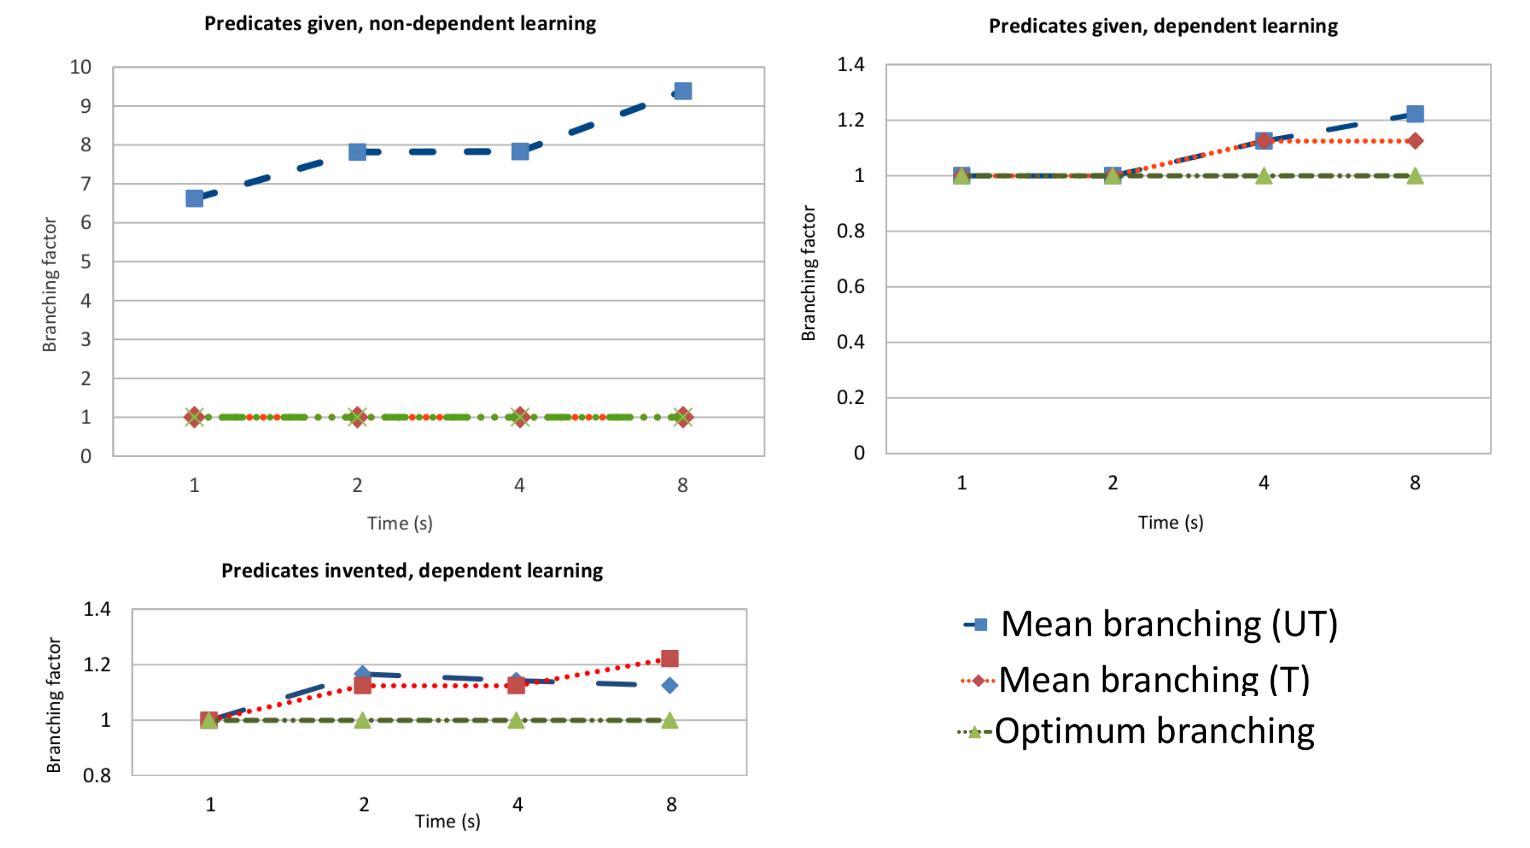
\includegraphics[width=0.8\textwidth]{experiments_1}}
    \caption{Mean branching factor $\rho$ for untyped (UT) and typed (T) MIL.
      Experiments are running on 15 proofs in CL. }
  \end{figure}
  \note[item]{
    Our first experiment considered determinism of typed MIL in comparison
    to untyped MIL. For each example we consider the branching factor ($\rho$) of the
    learned strategy, indicating the number of possible proof trees (including partial
    trees and failures) which could be constructed by applying the strategy to a goal.
    Branch points are found by manual inspection of the learned strategies. These
    occur when a goal could follow more than one edge in the graph, either through
    over-general wire predictes or edges with the same label. Automated extraction
    is not currently supported by PSGraph and is future work.
    In these first experiments we provided an explicitly-defined wire predicate
    clause for each goal in the background information, with the type label omitted
    in the untyped experiments. The experiments were repeated with different time
    limits (1, 2, 4 and 8 seconds).
  }
\end{frame}

\begin{frame}
  \frametitle{Results}
  These differences are due to how Metagol constructs its’ solutions.
  \vspace*{1cm}
  Consider a strategy consisting of repeated applications of a single tactic.
  \vspace*{1cm}
  \begin{itemize}
  \item Typed MIL forms this using the Loop rule.
  \item With untyped MIL there is no requirement to use psgraph clauses.
  \end{itemize}

  \note[item]{where both base and step cases must include psgraph clauses. These
    are formed using lifted tactic clauses with a wpred clause.}
  \note[item]{In
    untyped MIL there is no requirement to use psgraph clauses, and so a solution
    is found using tactic clauses with no wire predicates.}
  \note[item]{Consequently when a goal
    passes thTrough the node there is no wire predicate to direct it either towards
    the next tactic or around the loop, and so both must be tried. There is a similar
    issue whenever there are multiple outputs from a node, and it is this lack of
    pre-conditions which results in the higher $\rho$.}
\end{frame}

\begin{frame}
  \frametitle{Results}
  \begin{figure}[h]
    \centering
    \frame{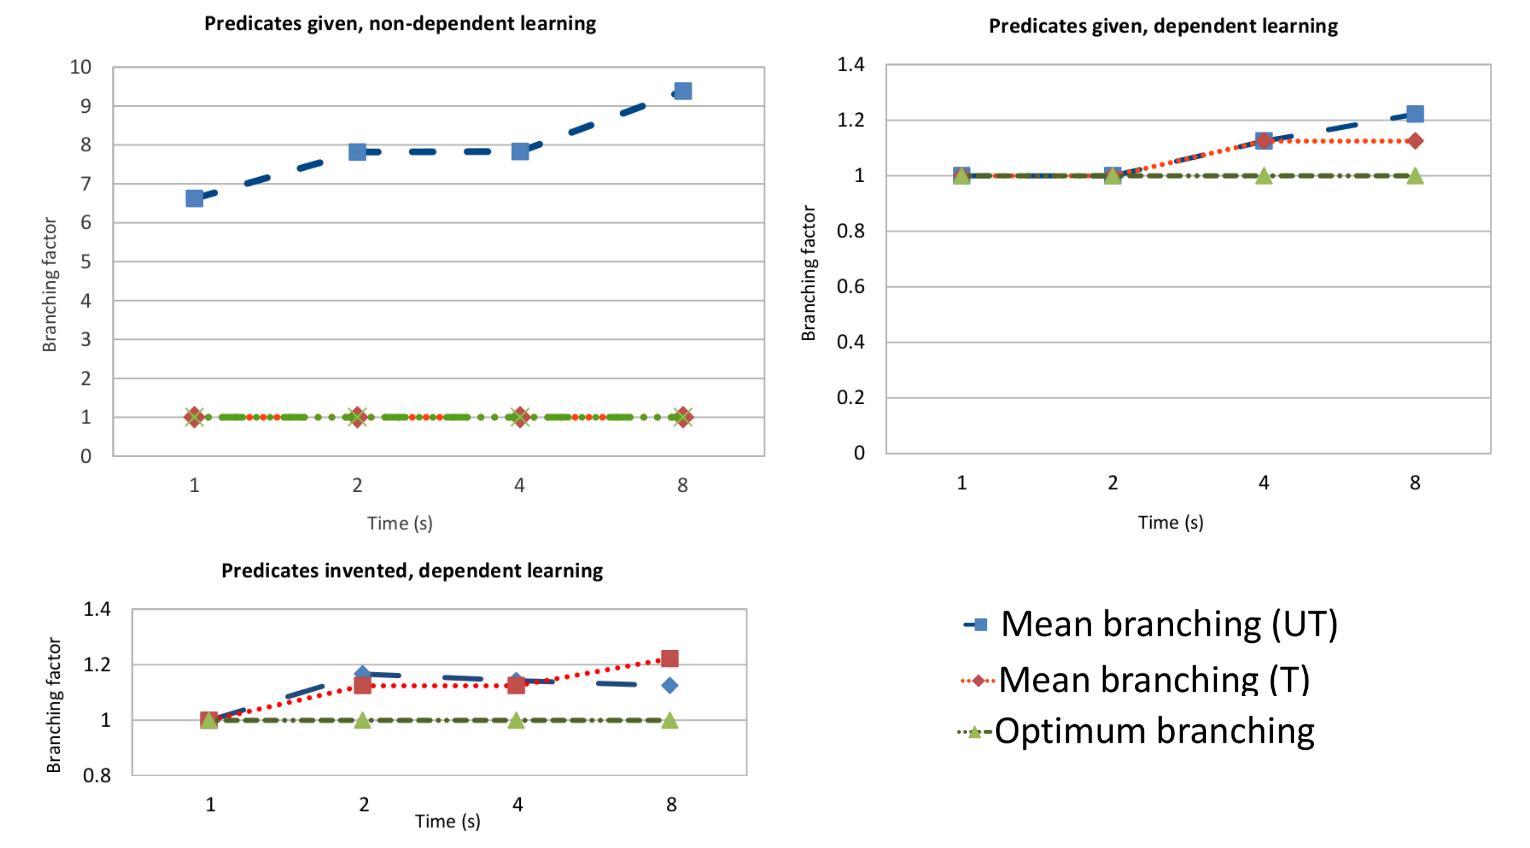
\includegraphics[width=0.8\textwidth]{experiments_1}}
    \caption{Mean branching factor $\rho$ for untyped (UT) and typed (T) MIL.}
  \end{figure}
  \note[item]{
    At first neither untyped nor typed MIL was able to learn from every example
    within the given time limit. This was due to the size of the solution required;
    the time needed grows exponentially with the number of clauses in the solution.
    In the untyped case this is less pronounced as the solutions are less detailed. In
    typed MIL a solution contains one clause for every lifted tactic plus a number of
    clauses describing how they link together, resulting in larger definitions for the
    same strategies. We address this by using dependent learning to learn smaller
    sub-strategies
  }
\end{frame}

\begin{frame}
  \frametitle{Dependent learning}
  \begin{figure}[h]
    \centering
    \frame{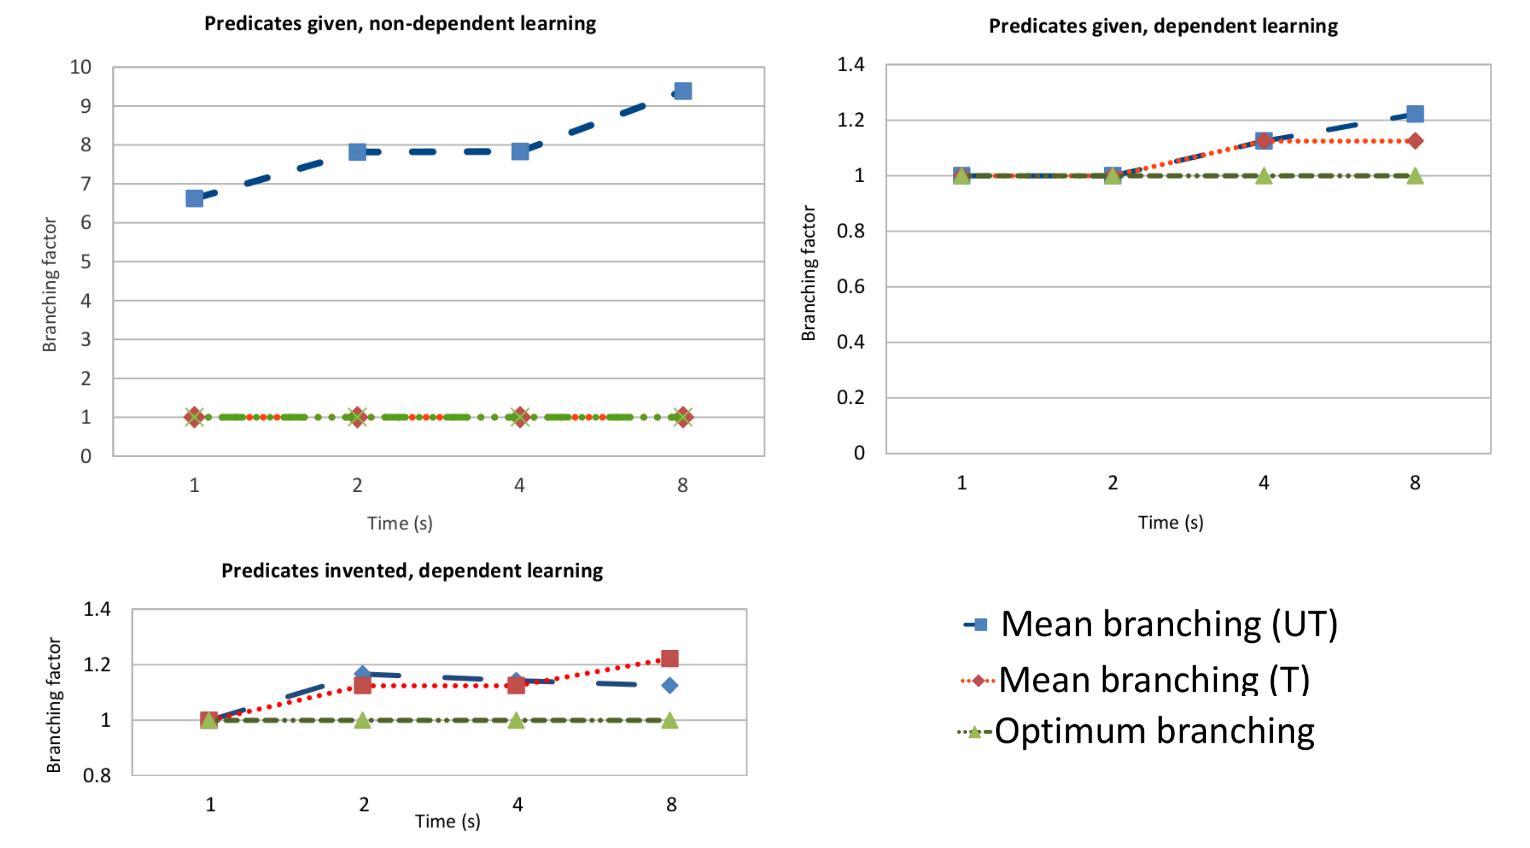
\includegraphics[width=0.8\textwidth]{experiments_1}}
    \caption{(Upper right) Smaller branching factor for UT.}
  \end{figure}
  \note[item]{
    By using dependent learning we reduce the time taken to learn more com-
    plex strategies, however this has the trade-off of taking longer to find simpler
    strategies. We have still not achieved 100\% success within the given time frame,
    nor are the additional strategies learned fully deterministic. However, there is a
    significantly smaller branching factor in the untyped case (Fig. 7, upper right).
    This is again due to Metagol’s construction of solutions: Metagol will always
    use the “simplest” (usually smallest) solution. When using dependent learning
    to learn sub-strategies describing sub-trees this means that the best
    metarule to use will generally be Chain, as each sub-strategy can then be extended one
    node at a time. Consequently there are fewer potential branch points for untyped
    MIL, while typed MIL is largely unaffected.

  }
\end{frame}

\begin{frame}
  \frametitle{Inventing pre-conditions}
  \begin{figure}[h]
    \centering
    \frame{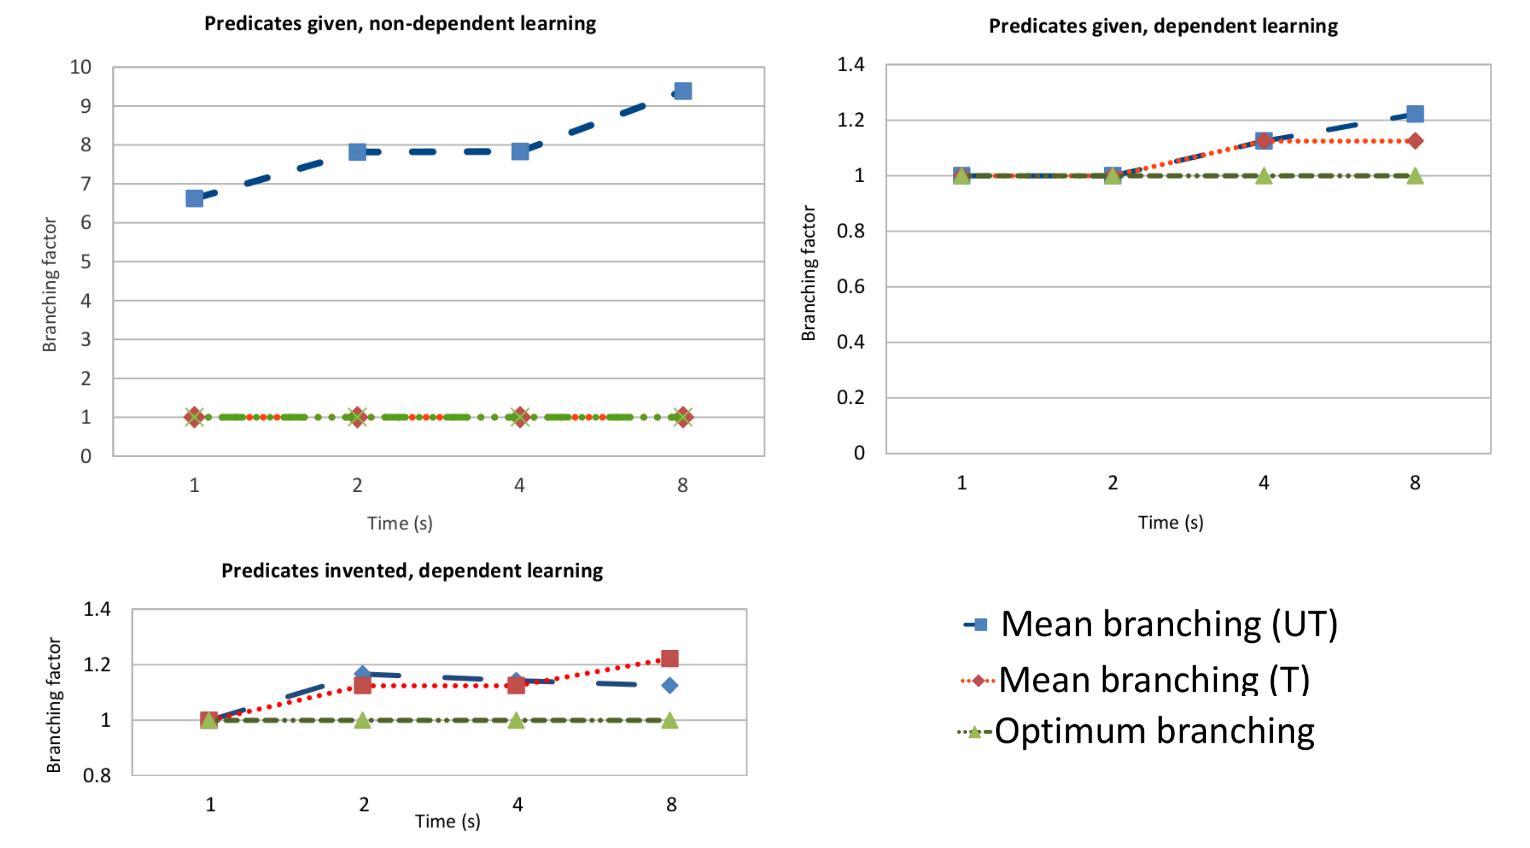
\includegraphics[width=0.8\textwidth]{experiments_1}}
    \caption{(Upper right) Smaller branching factor for UT.}
  \end{figure}
  \note[item]{The metarules restrict possible solutions, reflected in the weakening of the
    strategies seen here. Definitions are limited to using top symbol, hyp symbol,
    hyp and concl, which rules out other predicates being found. Since Metagol is
    forced to find a wpred clause in the typed case, and a simple monadic predicate in
    the untyped case, it must produce a definition which is too generalised and which
    would permit goals to follow an incorrect edge in the corresponding graph. Future
    work will include experiments using a minimal set of metarules from which others
    can be inferred, allowing Metagol to find better definitions for pre-conditions,
    including using the left( , )/right( , ) notation introduced in Definition 5.}
\end{frame}

\subsection[Conclusion]{Conclusion}

\begin{frame}
  \frametitle{Conclusion}
  \begin{enumerate}
  \item Show that MIL can learn proof strategies for the PSGraph language.
  \item Extend MIL with types.
  \item Demonstrate that ``typed MIL learns more deterministic proof strategies than untyped MIL''.
  \item Show that introducing dependent learning reduces the time taken to learn a strategy.
  \end{enumerate}
  \note[item]{
    Able to learn proof strategies from 86\% of the examples and thus supports
    that MIL is capable of learning proof strategies in
    our framework.}
  \note[item]{
    We have introduced types in the MIL
    framework by adding an additional constant argument to the predicate (C2).
  }
  \note[item]{
    The results show that typed MIL learns wire predicates and reduces branching,
    although we were able to learn strategies from fewer examples. Our assertion
    (C3) that typed MIL reduces non-determinism is distinct from success rate,
    however, and so is validated.
  }
  \note[item]{
    The introduction of types means a larger number
    of clauses to represent strategies, which increases the run time for Metagol and
    is the reason for failure in most cases. This is addressed through the use of
    dependent learning, and the slight increase in successful learning validates
    (C4).
  }
\end{frame}

\begin{frame}
  \frametitle{Further work}
  \begin{itemize}
  \item Improving learned strategies by using a combinator-based approach.
  \item Introducing combinators (such as OR and LOOP) to handle multiple outputs.
  \item Learn from higher order logic (predicate logic).
  \end{itemize}  
\end{frame}

\section[HOLStep]{HOLStep : A machine learning dataset for HOL theorem proving}

\subsection[Introduction]{Introduction and context}

\begin{frame}
  \frametitle{Introduction and context}
  Deep learning has proven to be a powerful tool for embedding semantic meaning
  and logical relationships into geometric spaces (CNN).
  \vspace*{1cm}
  \begin{itemize}
  \item AlphaGo
  \item Premise selection
  \item Automated translation
  \item ...
  \end{itemize}
\end{frame}

\begin{frame}
  \frametitle{Goal}
  \begin{itemize}
  \item Create a dataset for machine learning based on the proof steps (focus on
    HOL Light).
  \item Discuss the proof step classification tasks that can be attempted using the
    dataset.
  \item Propose baseline models.
  \item Evaluate the models.
  \end{itemize}
\end{frame}

\subsection[Dataset]{Dataset extraction}

\begin{frame}
  \frametitle{HOL Light}
  Focus on HOL Light for two reasons :
  \begin{itemize}
  \item follows the LCF approach.
  \item implements higher-order logic as its foundation.
  \end{itemize}

  \note[item]{This means that complicated inferences are reduced to the most primitive ones and the data extrac-
    tion related modifications can be restricted the primitive inferences and it is relatively easy to extract
    proof steps at an arbitrary selected level of granularity.}
  \note[item]{Second, HOL Light implements higher-order
    logic (Church, 1940) as its foundation, which on the one hand is powerful enough to encode most
    of today’s formal proofs, and on the other hand allows for an easy integration of many powerful
    automation mechanisms (Baader Nipkow, 1998; Paulson, 1999).}
\end{frame}

\begin{frame}
  \frametitle{Theorem selection}
  The theorems that are derived by most common proof functions are extracted by
  patching these functions.
  \vspace*{1cm}
  The remaining theorems are extracted from the underlying OCaml
  programming language interpreter.
\end{frame}

\begin{frame}
  \frametitle{Testing and training sets}
  Training and testing examples are grouped by proof, for each proof we have
  \begin{itemize}
  \item the conjecture.
  \item the dependencies of the theorem.
  \item list of used and not used intermediate statements.
  \end{itemize}
  \note[item]{This means that the conjectures used
    in the training and testing sets are normally disjoint.}
  \note[item]{In the dataset, for every proof we provide the same number of
    useful and non-useful steps. As such, the proof step classification problem
    is a balanced two-class classification problem, where a random
    baseline would yield an accuracy of 0.5.}
\end{frame}

\begin{frame}
  \frametitle{Statements}
  For each statements (conjecture, proof dependency, or intermediate statement)
  :
  \begin{itemize}
  \item human-like printout (with parenthesis).
  \item predefined tokenization.
  \end{itemize}

  \note[item]{The tokenization that we propose attempts to reduce the number of parentheses. To do this we
    compute the maximum number of arguments that each symbol needs to be applied to, and only mark
    partial application. This means that fully applied functions (more than 90\% of the applications) do
    not require neither application operators nor parentheses. Top-level universal quantifications are
    eliminated, bound variables are represented by their de Bruijn indices (the distance from the corre-
    sponding abstraction in the parse tree of the term) and free variables are renamed canonically. Since
    the Hindley-Milner type inference Hindley (1969) mechanisms will be sufficient to reconstruct the
    most-general types of the expressions well enough for automated-reasoning techniques Kaliszyk
    et al. (2015) we erase all type information.}
\end{frame}

\begin{frame}
  \frametitle{Statistics}
    \begin{figure}[h]
    \centering
    \frame{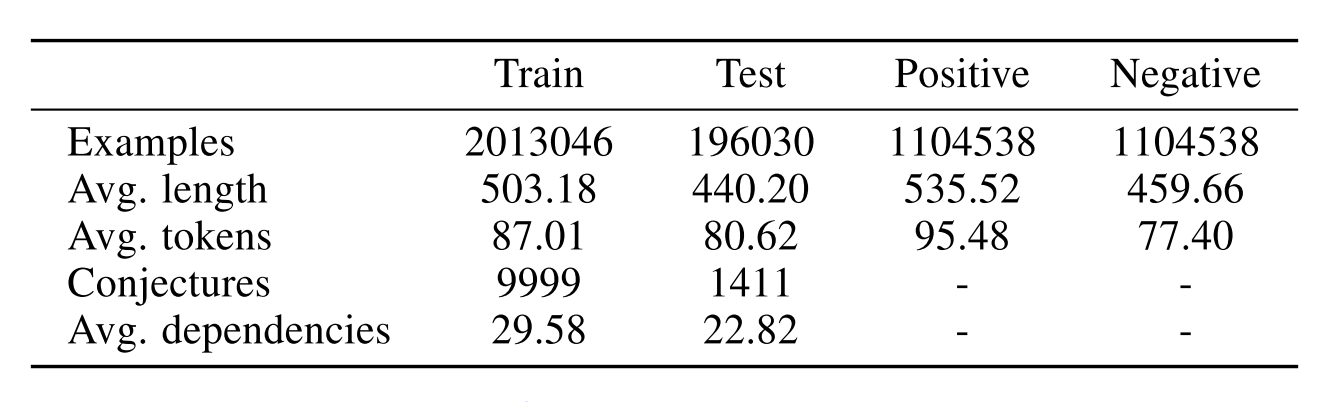
\includegraphics[width=0.8\textwidth]{stats}}
    \caption{HolStep dataset statistics.}
  \end{figure}
\end{frame}

\subsection[ML Tasks]{Machine Learning Tasks}

\begin{frame}
  \frametitle{Possible tasks}
  \begin{itemize}
  \item Predicting whether a statement is useful in the proof of a given conjecture;
  \item Predicting the dependencies of a proof statement (premise selection);
  \item Predicting whether a statement is an important one (human named);
  \item Predicting which conjecture a particular intermediate statement originates from;
  \item Predicting the name given to a statement;
  \item Generating intermediate statements useful in the proof of a given conjecture;
  \item Generating the conjecture the current proof will lead to. 
  \end{itemize}
\end{frame}

\begin{frame}
  \frametitle{Is a statement useful ?}
  Focus on the first task, which can be specialized into two different tasks :
  \begin{itemize}
  \item Unconditioned classification of proof steps.
  \item Conditioned classification of proof steps.
  \end{itemize}

  \note[item]{Unconditioned classification of proof steps: determining how likely a given proof is to be
    useful for the proof it occurred in, based solely on the content of statement (i.e. by only
    providing the model with the step statement itself, absent any context).}
  \note[item]{Conditioned classification of proof steps: determining how likely a given proof is to be
    useful for the proof it occurred in, with “conditioning” on the conjecture statement that the
    proof was aiming to attain, i.e. by providing the model with both the step statement and the
    conjecture statement).}
\end{frame}

\begin{frame}
  \frametitle{interaction with an ITP}
  Tasks that require most human time :
  \begin{itemize}
  \item the search for good intermediate steps.
  \item the search for automation techniques able to justify the individual steps.
  \item searching theorem proving libraries for the necessary simpler facts.
  \end{itemize}
  Corresponds to the machine learning tasks proposed previously.
  \note[item]{Being able
    to predict the usefulness of a statement will significantly improve many automation techniques.
    The generation of good intermediate lemmas or intermediate steps can improve level of granularity
    of the proof steps. Understanding the correspondence between statements and their names can
    allow users to search for statements in the libraries more efficiently (Aspinall and Kaliszyk, 2016).
    Premise selection and filtering are already used in many theorem proving systems, and generation
    of succeeding steps corresponds to conjecturing and theory exploration.}
\end{frame}

\subsection[NN Architecture]{Neural Network Architecture}

\begin{frame}
  \frametitle{Baseline models}
  For each tasks (conditioned and unconditioned classification) : three
  different deep learning architectures.
  \vspace*{1cm}
  Models are implemented in Tensorflow using the Keras framework.
  \note[item]{cover a range of architecture features (from convolutional networks
    to recurrent networks), aiming at probing what characteristics of the data are the most helpful for
    usefulness classification}
\end{frame}

\begin{frame}
  \frametitle{Unconditioned classification models}
  \begin{figure}[h]
    \centering
    \frame{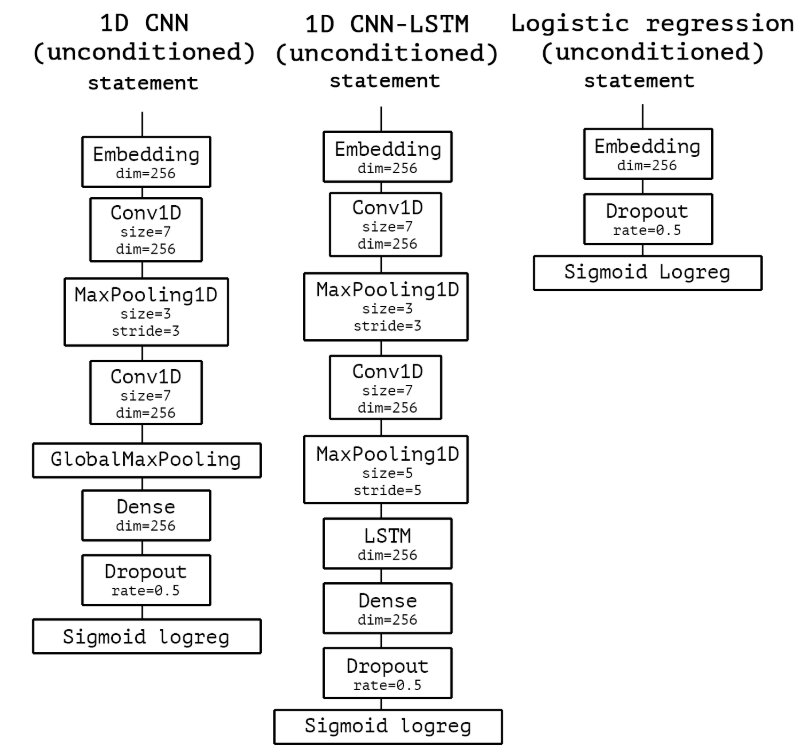
\includegraphics[width=0.6\textwidth]{models_1}}
    \caption{Unconditioned classification model architectures.}
  \end{figure}
  \note[item]{Logistic regression on top of learned token embeddings. This minimal model aims to
    determine to which extent simple differences between token distribution between useful
    and non-useful statements can be used to distinguish them. It provides an absolute floor on
    the performance achievable on this task.}
  \note[item]{2-layer 1D convolutional neural network (CNN) with global maxpooling for sequence re-
    duction. This model aims to determine the importance of local patterns of tokens.}
  \note[item]{2-layer 1D CNN with LSTM sequence reduction. This
    model aims to determine the importance of order in the features sequences.}
\end{frame}

\begin{frame}
  \frametitle{Conditioned classification models}
  \begin{figure}[h]
    \centering
    \frame{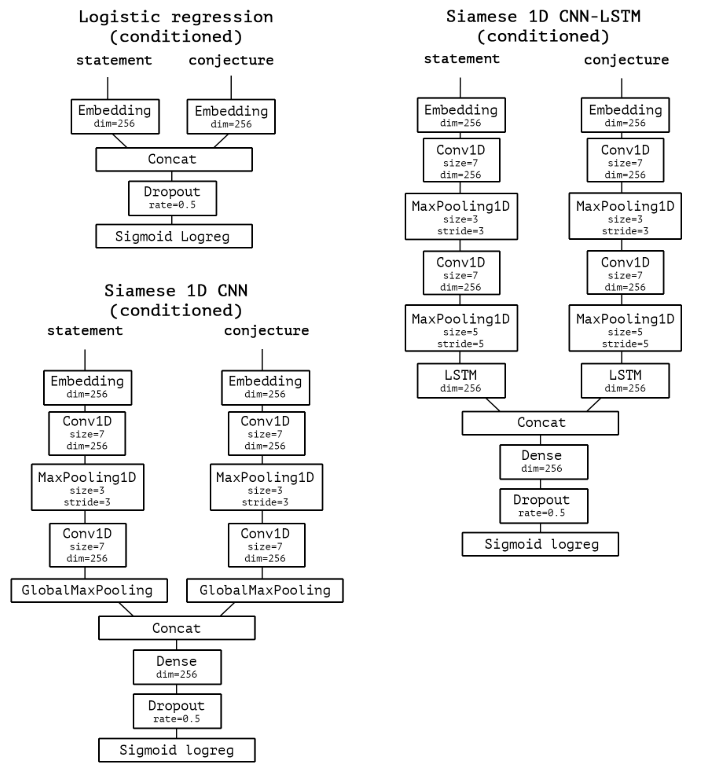
\includegraphics[width=0.5\textwidth]{models_2}}
    \caption{Conditioned classification model architectures.}
  \end{figure}

  \note[item]{
    For this task, we use versions of the above models that have two siamese branches (identical branches
    with shared weights), with one branch processing the proof step statement being
    considered, and the other branch processing the conjecture. Each branch
    outputs an embedding; these two embeddings (step embedding and conjecture
    embedding) are then concatenated and the classified by a fully-
    connected network. See figure 2 for a layer-by-layer description of these models.
  }
\end{frame}

\begin{frame}
  \frametitle{Input statement encoding}
  Two types of encoding :
  \begin{itemize}
  \item Character-level encoding of the human-readable versions of the
    statements.
  \item Token-level encoding of the versions of the statements.
  \end{itemize}
  \note[item]{It should be noted that all of our models start with an Embedding
    layer, mapping tokens or characters in the statements to dense vectors in a
    low-dimensional space. We consider two possible encodings for presenting the
    input statements (proof steps and conjectures) to the Embedding layers of
    our models:}
  \note[item]{Character-level encoding of the human-readable versions of the statements, where each
    character (out of a set of 86 unique characters) in the pretty-printed statements is mapped
    to a 256-dimensional dense vector. This encoding yields longer statements (training state-
    ments are 308 character long on average).}
  \note[item]{Token-level encoding of the versions of the statements rendered with our proposed high-
    level tokenization scheme. This encoding yields shorter statements (training statements are
    60 token long on average), while considerably increasing the size of set of unique tokens
    (1993 total tokens in the training set).}
\end{frame}

\subsection[Results]{Results}

\begin{frame}
  \frametitle{Results : architecture}
  \begin{figure}[h]
    \centering
    \frame{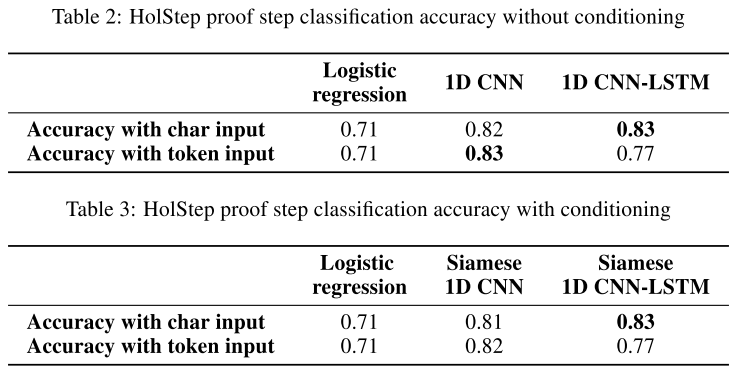
\includegraphics[width=0.8\textwidth]{results}}
  \end{figure}
  \note[item]{unconditioned 1D CNN model yields an accuracy of 82% to 83%, both with char-
    acter encoding and token encoding (tables 2 and 3). This demonstrates that patterns of characters or
    patterns of tokens are considerably more informative than single tokens for the purpose of usefulness
    classification}
  \note[item]{Finally, our unconditioned convolutional-recurrent model does not improve upon the results of the
    1D CNN, which indicates that our models are not able to meaningfully leverage order in the feature
    sequences into which the statements are encoded.}
\end{frame}

\begin{frame}
  \frametitle{Results : input encoding}
  \begin{figure}[h]
    \centering
    \frame{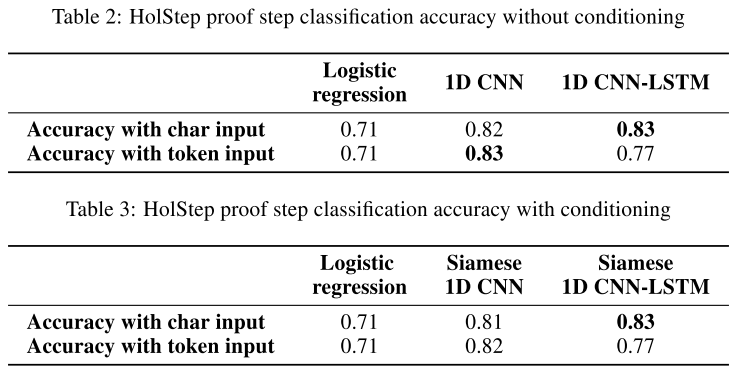
\includegraphics[width=0.8\textwidth]{results}}
  \end{figure}
  \note[item]{For the logistic regression model and the 2-layer 1D CNN model, the choice of input encoding seems
    to have little impact. For the convolutional-recurrent model, the use of the high-level tokenization
    seems to cause a large decrease in model performance (figs. 4 and 6). This may be due to the fact
    that token encoding yields shorter sequences, making the use of a LSTM less
    relevant.}
\end{frame}

\begin{frame}
  \frametitle{Results : conditioning}
  \begin{figure}[h]
    \centering
    \frame{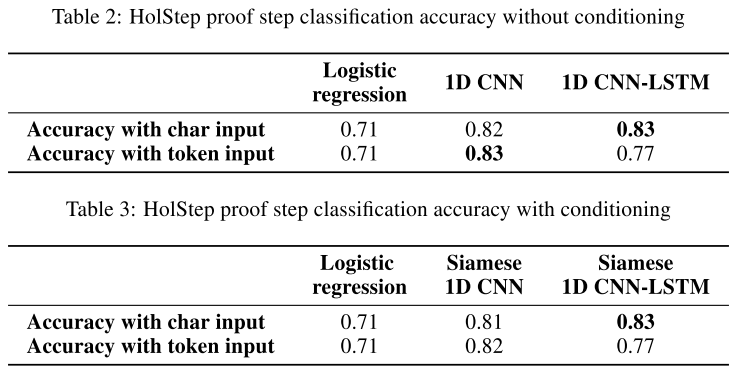
\includegraphics[width=0.8\textwidth]{results}}
  \end{figure}
  \note[item]{None of our conditioned models appear to be able to improve upon the unconditioned models, which
    indicates that our architectures are not able to leverage the information provided by the conjecture.
    The presence of the conditioning does however impact the training profile of our models, in partic-
    ular by making the 1D CNN model converge faster and overfit significantly quicker (figs. 5 and 6).}
\end{frame}

\subsection[Conclusion]{Conclusion}

\begin{frame}
  \frametitle{Conclusion}
  \begin{itemize}
  \item The baseline deep learning models is fairly weak, but still able to
    predict statement usefulness.
  \item Not able to leverage order in the input sequences, nor conditioning on
    the conjectures.
  \item No formal reasoning.
  \item Use pattern matching on tokens and characters.
  \item Improvement : HOL graph structure.
  \end{itemize}
\end{frame}

\begin{frame}
  \frametitle{Future work}
  \begin{itemize}
  \item Focus on more ITP and ATP.
  \item Premise selection and intermediate sentence generation.
  \end{itemize}
\end{frame}

\section[Conclusion]{Conclusion}

\begin{frame}
\frametitle{References}
\printbibliography
\end{frame}

\end{document}